\chapter{Working title}
\label{sec:something}


Throughout the duration of this study, we have carried out a great number of DFT calculations in order to present an comprehensive overview of promising high-entropy silicides. In payment to the thermoelectric prospect of hexagonal $Fe_2Si$, we firstly attempted to build SQSs from this structure. However, in agreement to the experimental indication that \textbf{cite?}, 3d silicides adopt a metallic character when the 3d elements supercede $50\%$ of the composition, all of our SQSs displayed a clear absence of an energy gap between the valence band and conduction band, we will return  more specifically to these compositions later in this section. For now, we will present the results of a much more interesting and promising case, in which we replaced $Fe_2Si$, with $\beta-FeSi_2$, effectively doubling the Si-metal ratio. Hence why we prefer the term high-entropy silicides more so than high-entropy alloys, as these particular compositions does not lie directly within the conditions presented in sections (\textbf{HEA}). In this structure, we completed in total calculations regarding 17 distinct compositions and permutations, such $\text{ALLOY}Si_2$ SQS based on CoCrFeni, CrFeMnNi, CoCrMnNi, CrFeMnTi, CrFeTiNi, and permutations wihin these such as increasing or decreasing the distribution of certain elements. Of the 17 variants, each consists of 5 unique SQSs, and trialed with numerous functionals, magnetic configurations and other parameters, as discussed in section .., in attempt to locate the overall most stable and reliable results. With this approach, the complete number of calculations and results both escalated very quikly, therefore, in the intent of presenting a clear and informative report of the study, we will begin this section by analyzing the overall most promising structure, then present and discuss these results in relation to the remaining permutations and structures.    

The aforementioned system is composed of Cr, Fe, Mn, and Ni, equally distributed in a 48 atom SQSs of $FeSi_2$, wheras 32 of these is silicon atoms. Here after, this system will be abbreviated CFMN (fesi2) to spcify that its within the framework of the cmce $FeSi_2$ unit cell.
 
The 5 distinct SQS can be seen in figure (method/SQS). Bellow, in table \ref{tab:FeSi2/CrFeMnNi_equal} we present a summary of the total energy, final magnetic moment and band gap corresponding to the 5 SQSs called A, B, C, D, and E respectfully. From a first glance, we observe very similar properties between the structures. The total energy per atom vary by $0.0092$ eV from the most stable structure C ($-6.6063$ eV) to the least stable structure D ($-6.6155$ eV). Similarly, the final magnetic moment is near identical throughout the span of SQSs, which is excepted given that aside from the unique distribution, all 5 SQSs contain the same amount and type of elements. On the contrary to the magnetic moment, the band gap is very sensitive to the type of SQS, ranging from a highest $0.05$ eV in structure B to $0$, ie nonexistent in structure D. A band gap in this range means for excellent application as thermoelectric materials. 


\begin{table}[H]
\centering
\begin{tabular}{@{}cccc@{}}
\toprule
Structure  & Total energy/atom (eV) & Final magnetic moment (?) & Band gap (eV) \\ \midrule
\textbf{A} & −6,6080                & 4.0006                    & 0.0280        \\
\textbf{B} & −6,6138                & 3.9999                    & 0.0523        \\
\textbf{C} & −6,6063                & 4.0008                    & 0.0344        \\
\textbf{D} & −6,6155                & 4.0001                    & 0             \\
\textbf{E} & −6,6089                & 4.0000                    & 0.0495        \\ \bottomrule
\end{tabular}
\caption{Total energy per atom, final magnetic moment, and band gap (GGA) of 5 $Cr_4Fe_4Mn_4Ni_4Si_{32}$ SQSs based on $FeSi_2$}
\label{table:fesi2_summary}
\end{table}  
Furthermore regarding the band gaps, we note that the gaps are indirect, the specific transitions is listed bellow.

\begin{table}[H]
\centering
\begin{tabular}{@{}ccc@{}}
\toprule
Structure  & Gap (D/I) & Transition                              \\ \midrule
\textbf{A} & I         & (0.500,0.333,0.500)-(0.500,0.000,0.000)  \\
\textbf{B} & I         & (0.250,0.000,0.250)-(0.000,0.000,0.000)  \\
\textbf{C} & -         & (0.500,0.000,0.500)-(-0.250,0.333,0.500) \\
\textbf{D} & I         & -                                        \\
\textbf{E} & I         & (0.000,0.000,0.000)-(0.250,0.000,0.250)  \\ \bottomrule
\end{tabular}
\caption{Band gap transition of CFMN (fesi2) SQSs with PBE functional}
\end{table}

In this regard, it would have been very instructive to plot a band structure diagram to further evaluate the energy bands, however due to the complex nature of the SQSs and the implementation with TDEP we were not able to plot the bandstructure. Thus, in this section we will analyze the band gap by other meassures. The first method we will employ is to observe the band gap from the plotted density of states, in figure \textbf{ref bellow}. From these figures, we can determine the band gap from the distance in energy around the Fermi energy (here set to 0), where the density of states is exactly 0, in addition we can observe the band gap for spin $\uparrow$ (positive) and $\downarrow$ (negative) states.   

\begin{figure}[H]
	\centering
	\begin{subfigure}{0.9\textwidth}
		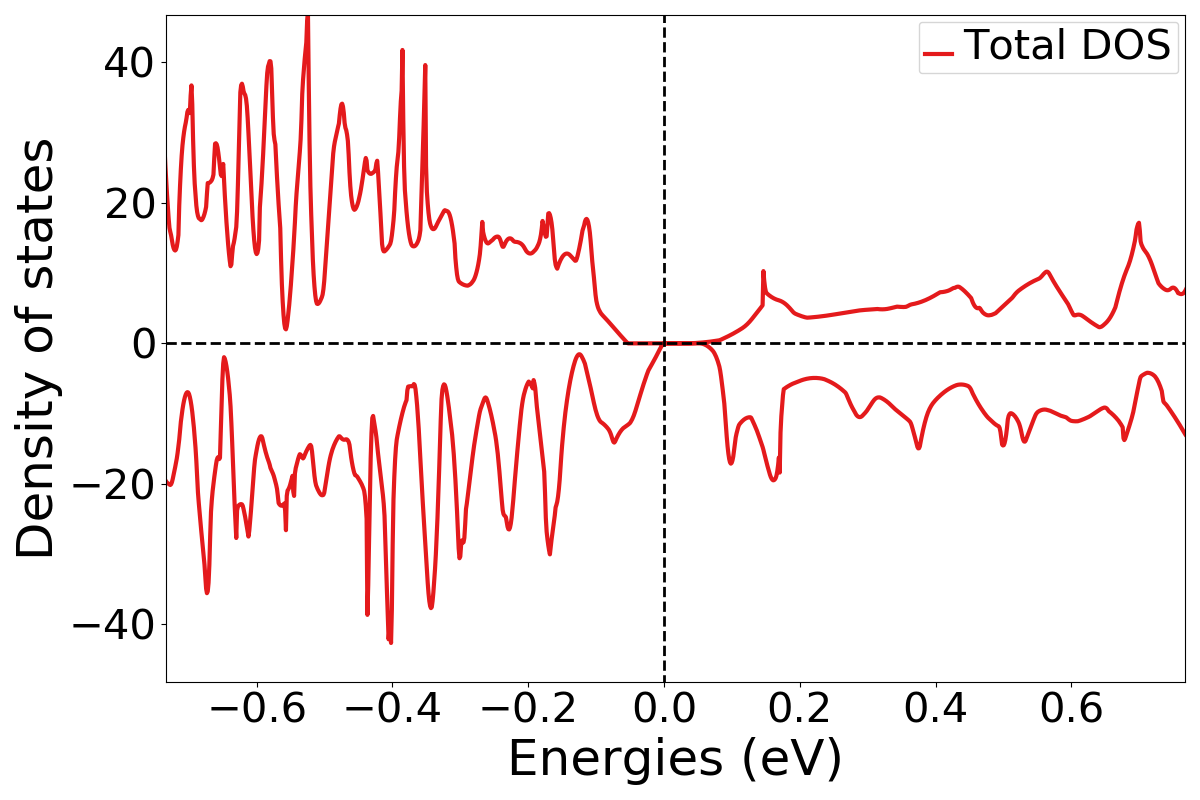
\includegraphics[width=\textwidth]{results/fesi2/DOS_A_toten.png}
	\end{subfigure}

	\begin{subfigure}{0.9\textwidth}
		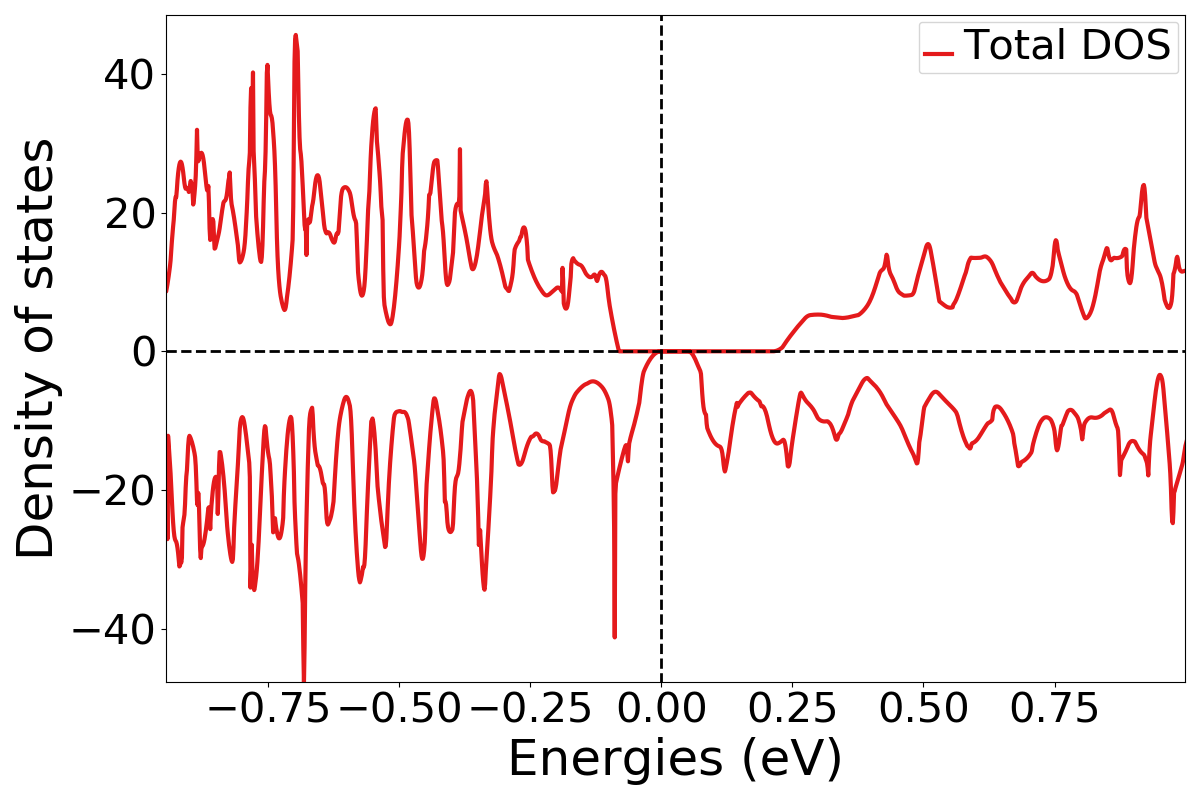
\includegraphics[width=\textwidth]{results/fesi2/DOS_B_toten.png}
	\end{subfigure}
	\begin{subfigure}{0.9\textwidth}
		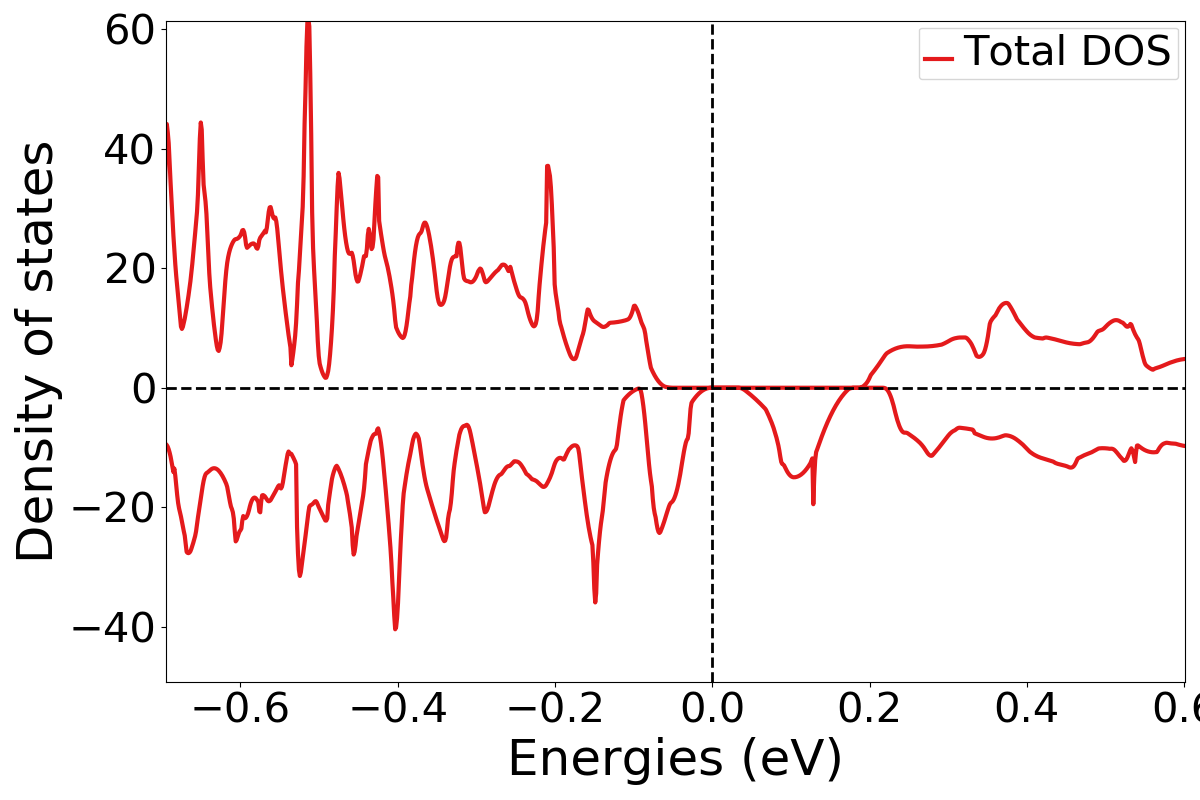
\includegraphics[width=\textwidth]{results/fesi2/DOS_C_toten.png}
	\end{subfigure}
\end{figure}
\begin{figure}[H]
	\centering
	\begin{subfigure}{0.9\textwidth}
		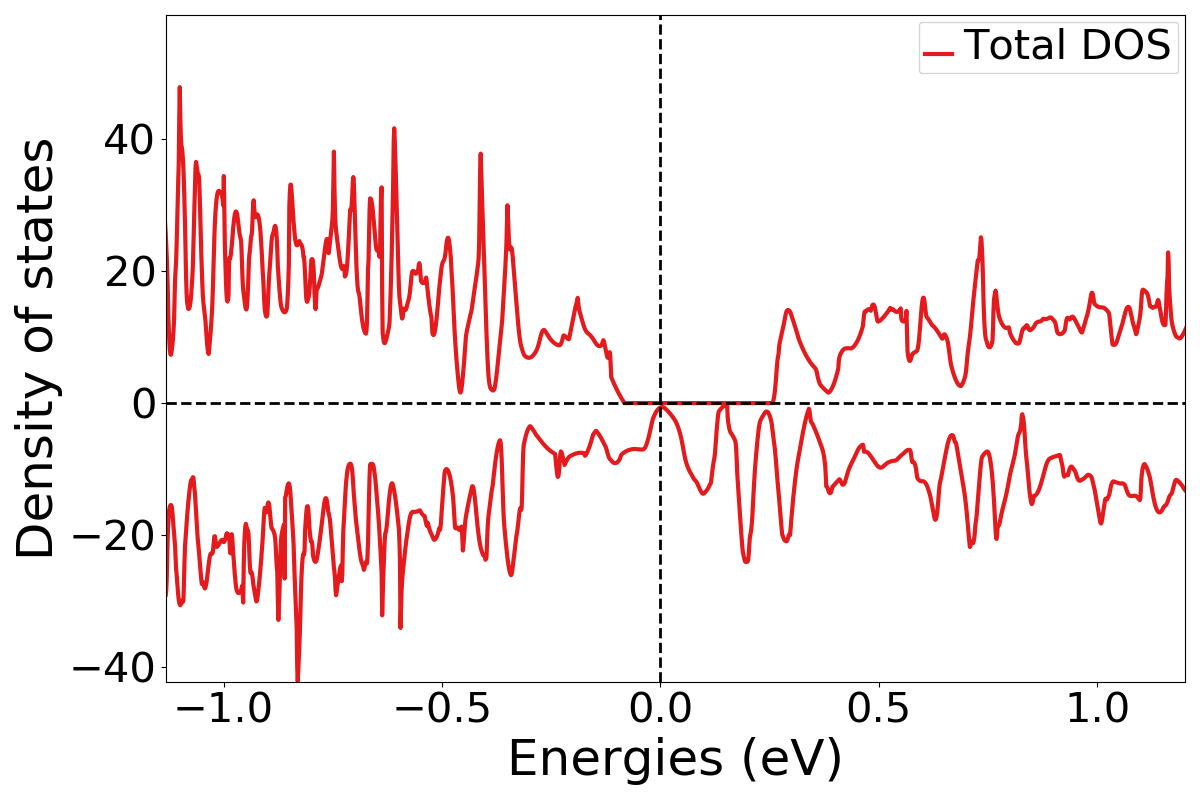
\includegraphics[width=\textwidth]{results/fesi2/DOS_D_toten.png}
	\end{subfigure}
	\begin{subfigure}{0.9\textwidth}
		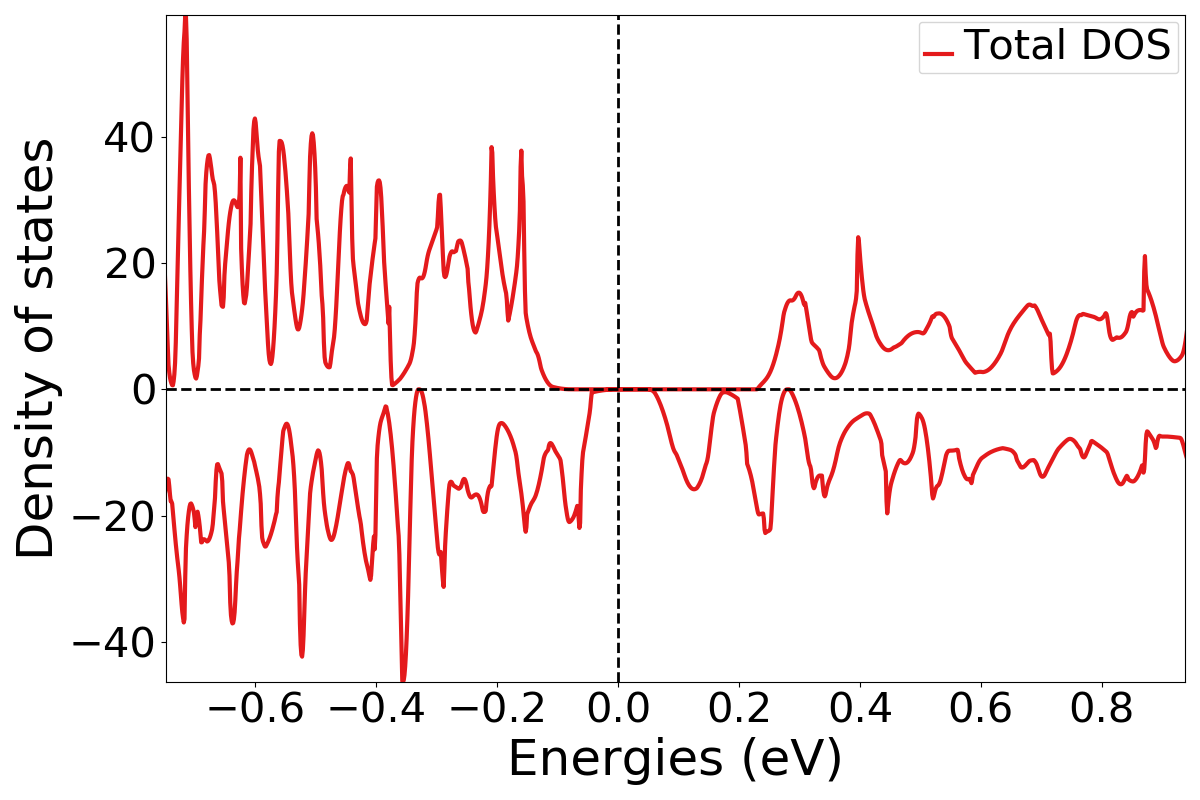
\includegraphics[width=\textwidth]{results/fesi2/DOS_E_toten.png}
	\end{subfigure}
	\caption{Density of states for structure A, B, C, D, E of $CFMNSi_2 (FeSi_2)$ SQSs (PBE GGA)}
	\label{dos_fesi2_gga}
\end{figure}



\begin{comment}
\begin{table}[H]
\centering
\begin{tabular}{@{}cccc@{}}
\toprule
Structure  & Spin-up & Spin-down & Total  \\ \midrule
\textbf{A} & 0.0814  & 0.0522    & 0.0281 \\
\textbf{B} & 0.2932  & 0.0523    & 0.0523 \\
\textbf{C} & 0.2355  & 0.0343    & 0.0343 \\
\textbf{D} & 0.3386  & 0         & 0      \\
\textbf{E} & 0.3078  & 0.0495    & 0.0495 \\ \bottomrule
\end{tabular}
\caption{Band gap (GGA) in spin up and spin down channels of CFMNSi2 structures}
\end{table}

\begin{table}[H]
\centering
\begin{tabular}{@{}cccc@{}}
\toprule
Structure  & PBE    & SCAN   & HSE06  \\ \midrule
\textbf{A} & 0.0281 & 0.0000 & 0.0207 \\
\textbf{B} & 0.0523 & 0.0890 & 0.1808 \\
\textbf{C} & 0.0344 & 0.0690 & 0.0196 \\
\textbf{D} & 0.0000 & 0.0000 & 0.0000 \\
\textbf{E} & 0.0495 & 0.1048 & 0.0133 \\ \bottomrule
\end{tabular}
\caption{Band gap of $CFMN (FeSi_2)$ SQSs with GGA (PBE), meta-GGA (SCAN) and hybrid-functionals (HSE06). \textbf{Add footnote to explain the uncertainty in these results regarding smearing type and width, and DOS and EIGENVAL}}
\end{table}
\end{comment}

\textbf{DOS analyse}

\begin{figure}[H]
\centering
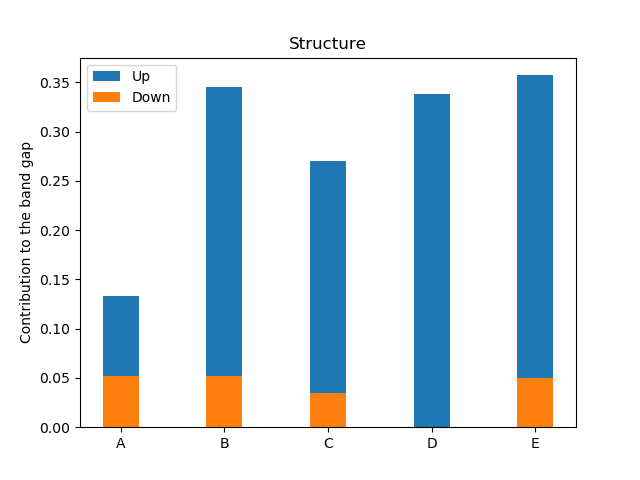
\includegraphics[scale=.7]{results/fesi2/spin_gap.png}
\caption{Band gap of CFMN fesi2 SQSs in spin up and spin down with PBE functional.}
\label{DOS_hse06_B}
\end{figure}

\textbf{Intro LDOS}

\textbf{Diskusjon LDOS}

\begin{figure}[H]
%\centering
	\begin{subfigure}{\textwidth}
		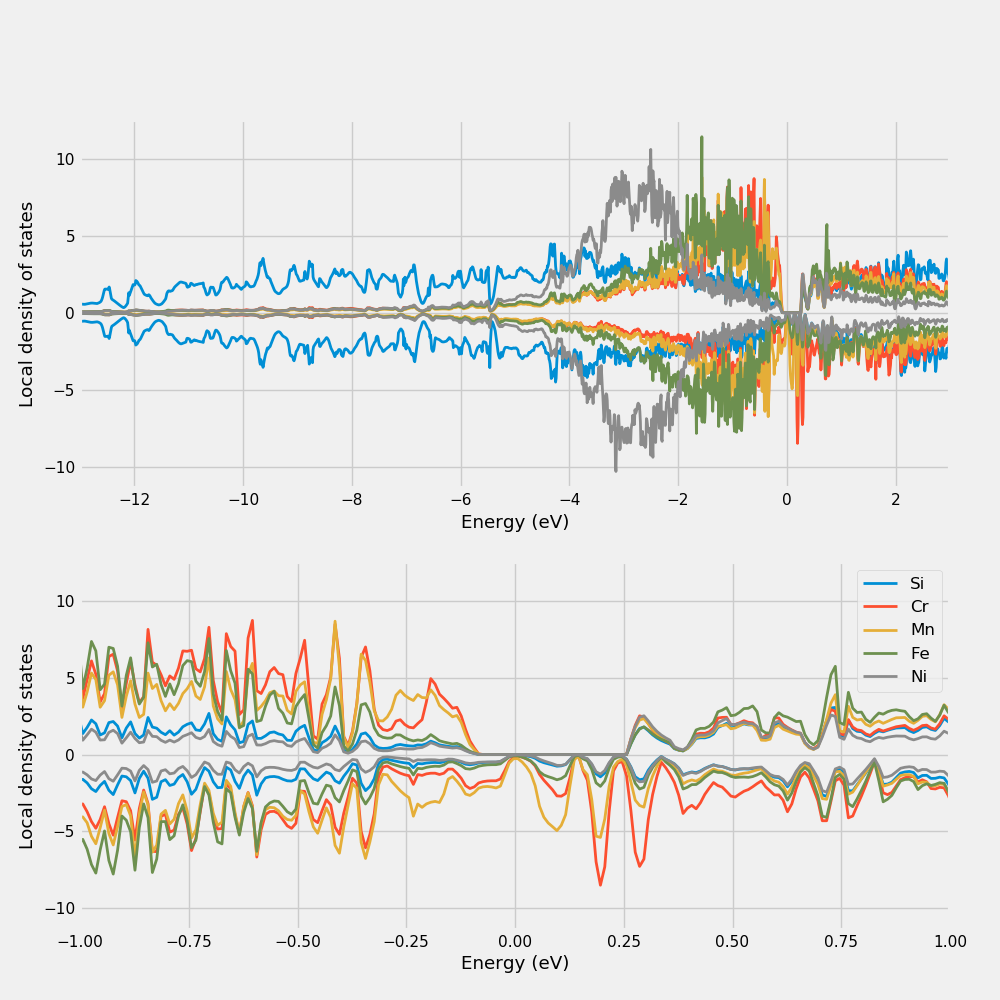
\includegraphics[width=\textwidth]{results/fesi2/A_LDOS.png}
		\caption{A}
	\end{subfigure}
	\begin{subfigure}{\textwidth}
		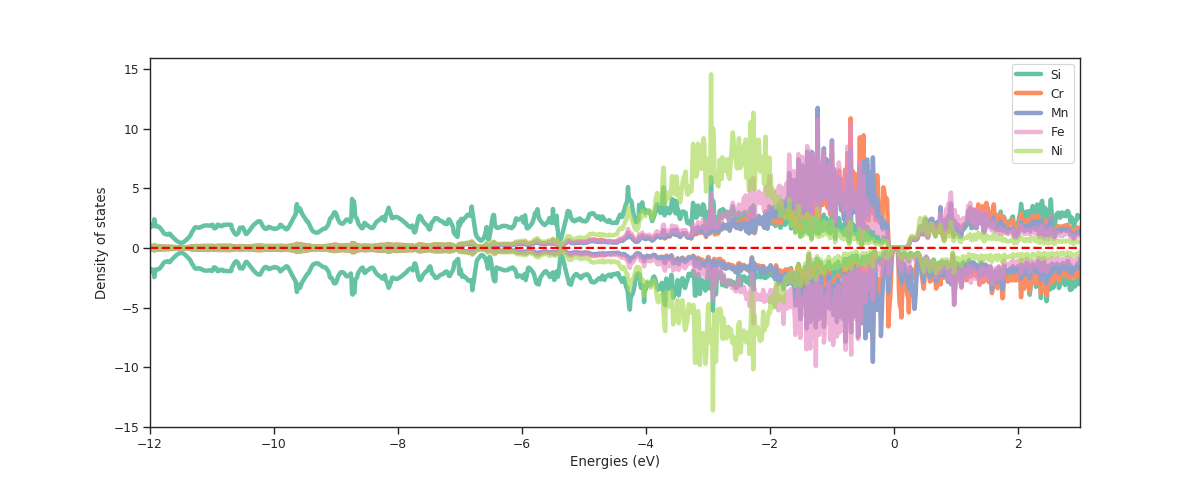
\includegraphics[width=\textwidth]{results/fesi2/B_LDOS.png}
		\caption{B}
	\end{subfigure}
	\begin{subfigure}{\textwidth}
		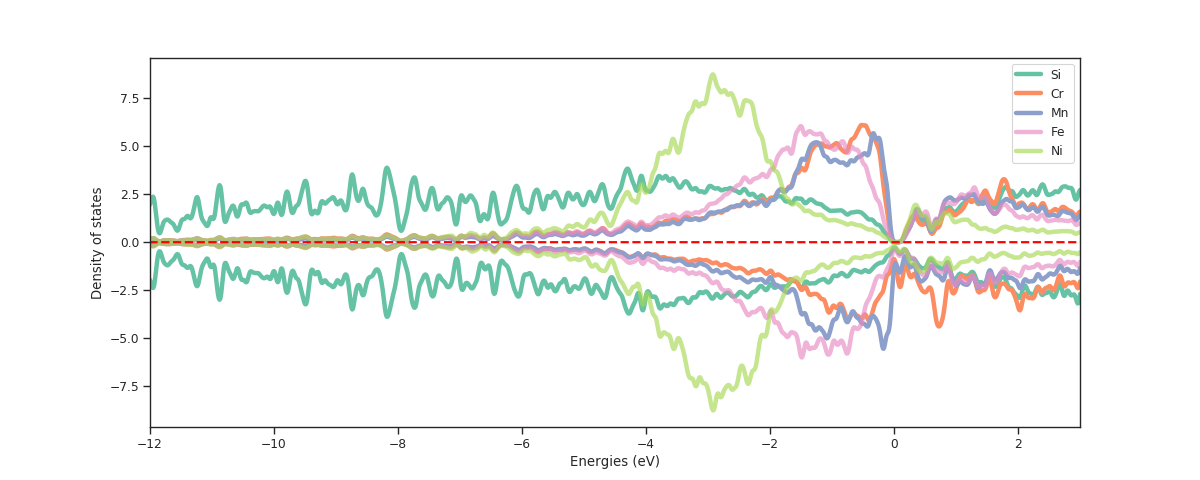
\includegraphics[width=\textwidth]{results/fesi2/C_LDOS.png}
		\caption{C}
	\end{subfigure}
	\begin{subfigure}{\textwidth}
		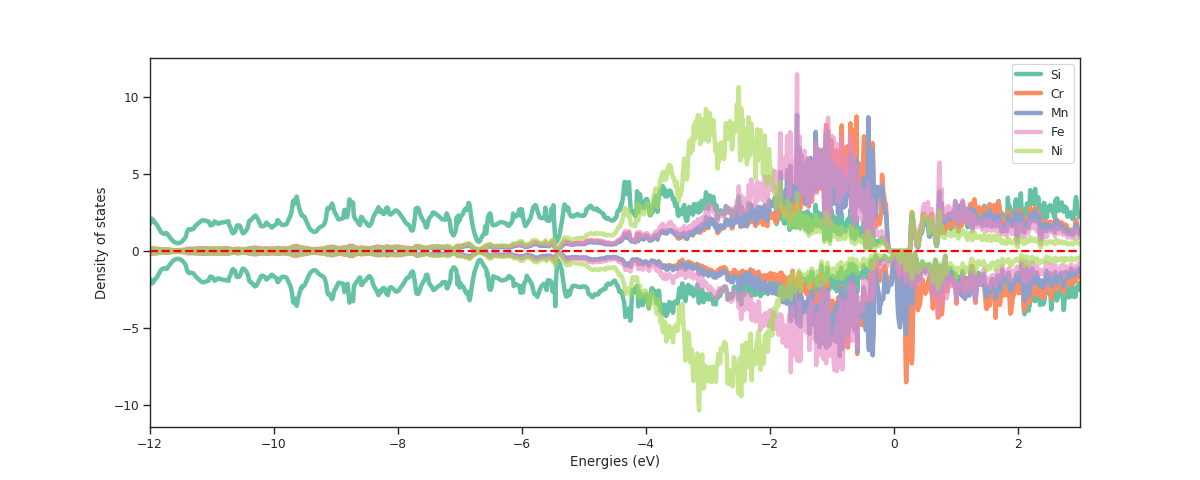
\includegraphics[width=\textwidth]{results/fesi2/D_LDOS.png}
		\caption{D}
	\end{subfigure}
\end{figure}		
\begin{figure}[H]
	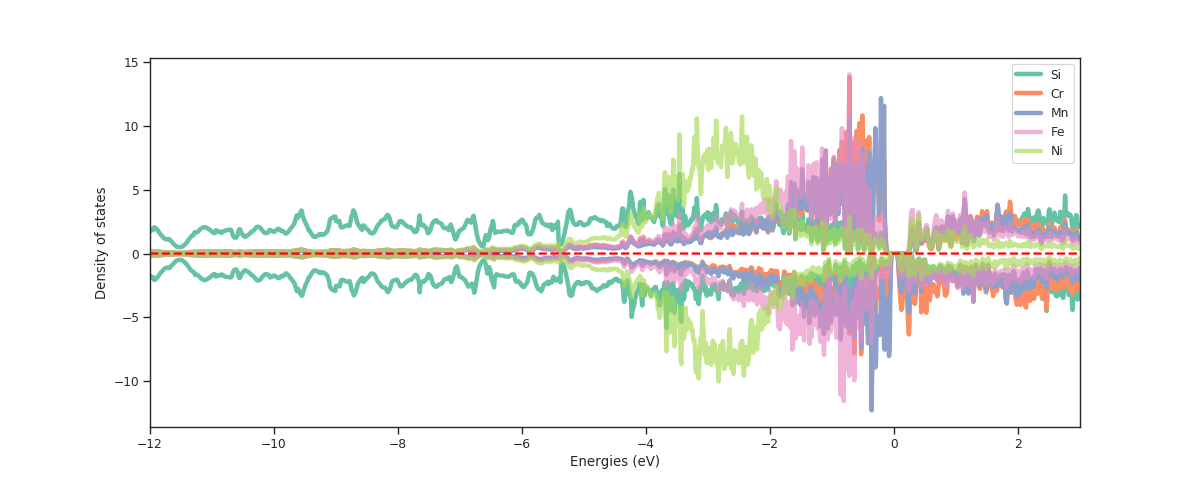
\includegraphics[width=\textwidth]{results/fesi2/E_LDOS.png}
	\caption{E}
\end{figure}

\textbf{Continue discussion LDOS, introduce and discuss PDFs}

\begin{figure}[H]
%\centering
	\begin{subfigure}{\textwidth}
		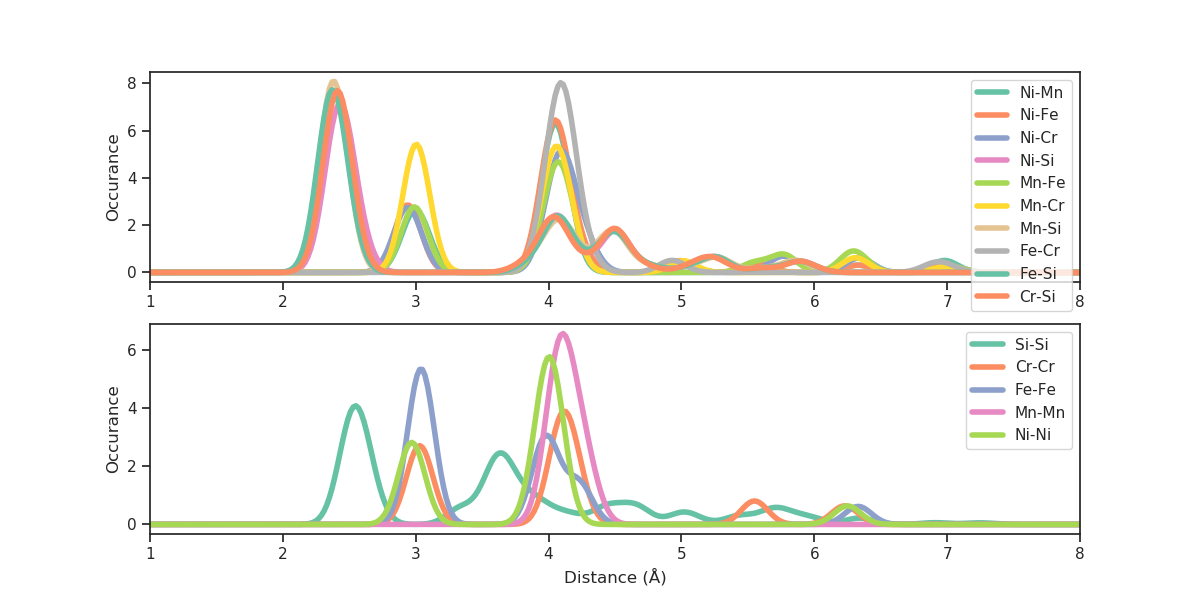
\includegraphics[width=\textwidth]{results/fesi2/A_PDF.png}
		\subcaption{A}
	\end{subfigure}	
	\begin{subfigure}{\textwidth}
		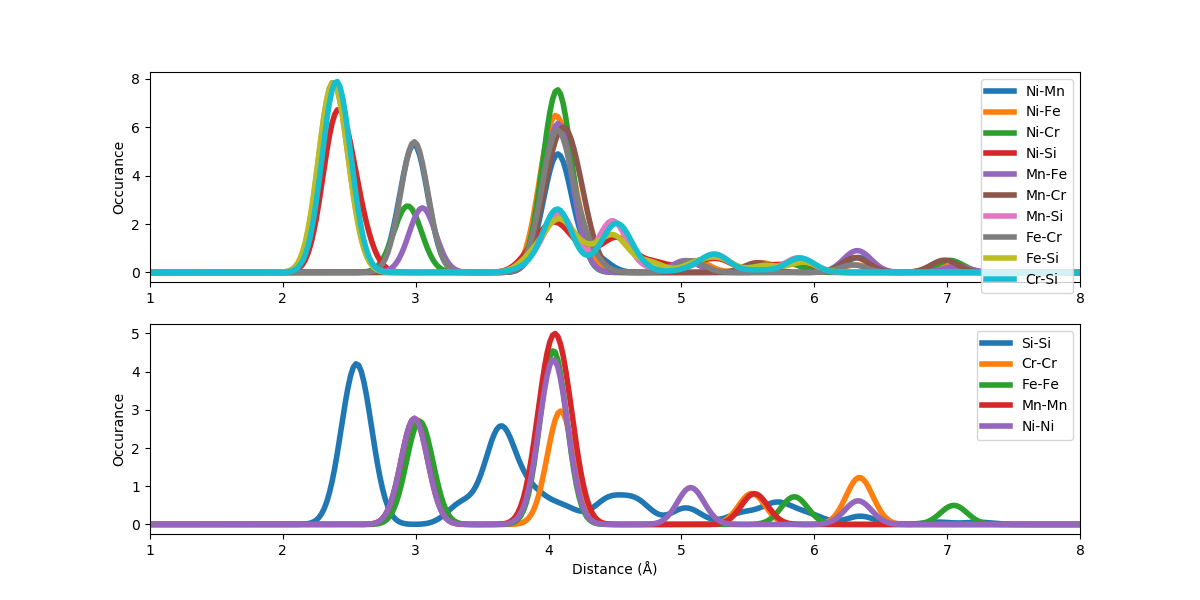
\includegraphics[width=\textwidth]{results/fesi2/B_PDF.png}
		\subcaption{B}
	\end{subfigure}
	\begin{subfigure}{\textwidth}
		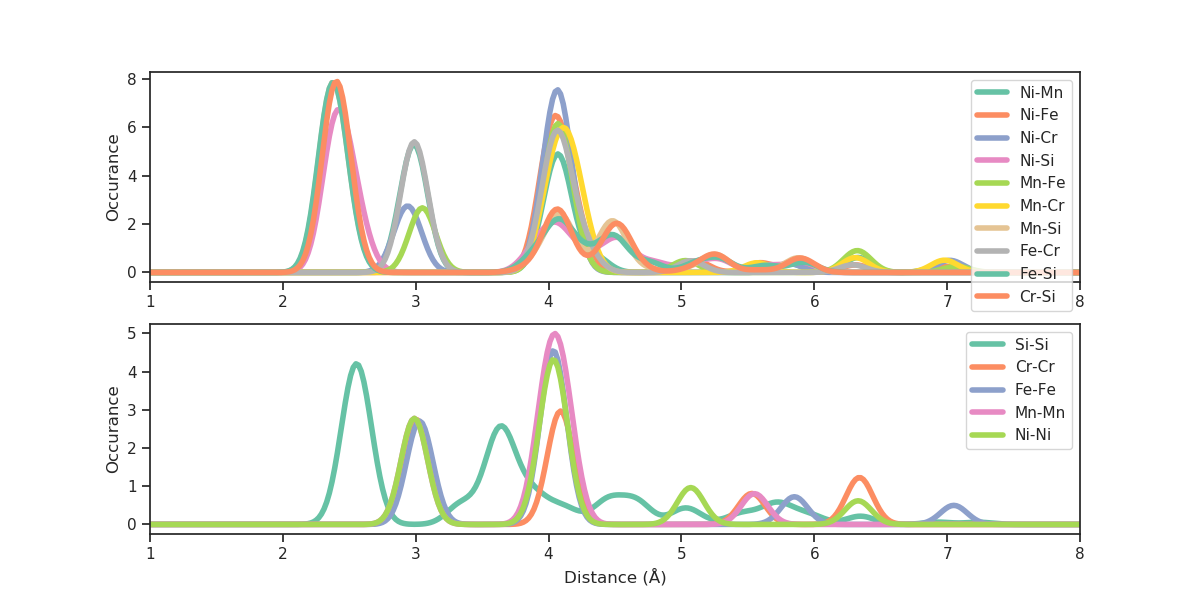
\includegraphics[width=\textwidth]{results/fesi2/C_PDF.png}
		\subcaption{C}
	\end{subfigure}
\end{figure}
\begin{figure}[H]
	\begin{subfigure}{\textwidth}
		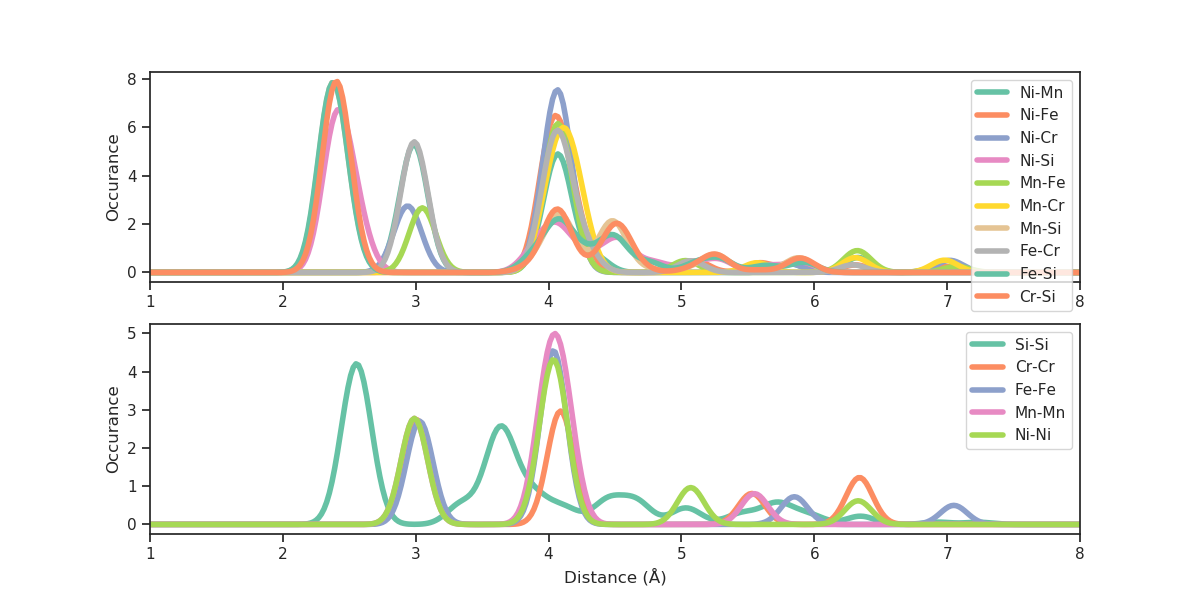
\includegraphics[width=\textwidth]{results/fesi2/D_PDF.png}
		\subcaption{D}
	\end{subfigure}
	\begin{subfigure}{\textwidth}
		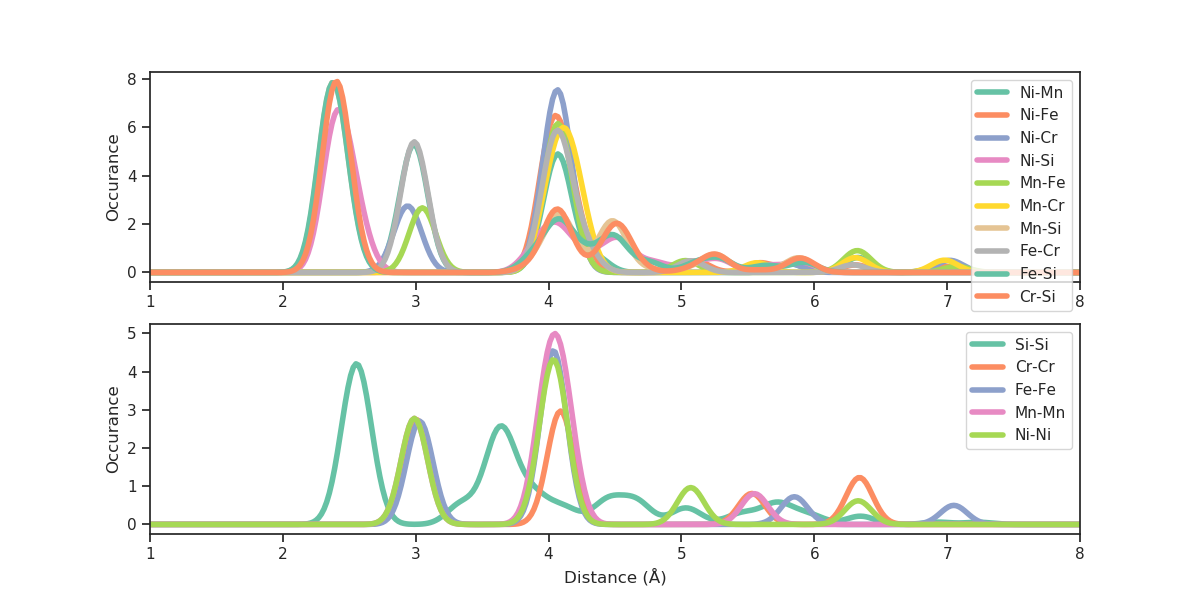
\includegraphics[width=\textwidth]{results/fesi2/E_PDF.png}
		\subcaption{E}
	\end{subfigure}
\end{figure}

\textbf{Finish discussion pdfs, introduce CHGCAR}

\begin{figure}
	\begin{subfigure}{0.5\textwidth}
		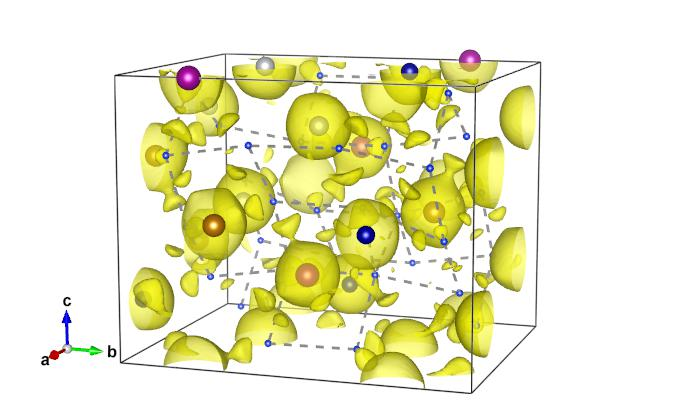
\includegraphics[width=\textwidth]{results/fesi2/A_CHGCAR.jpg}
		\caption{Structure A}
	\end{subfigure}
	\hfill
	\begin{subfigure}{0.5\textwidth}
		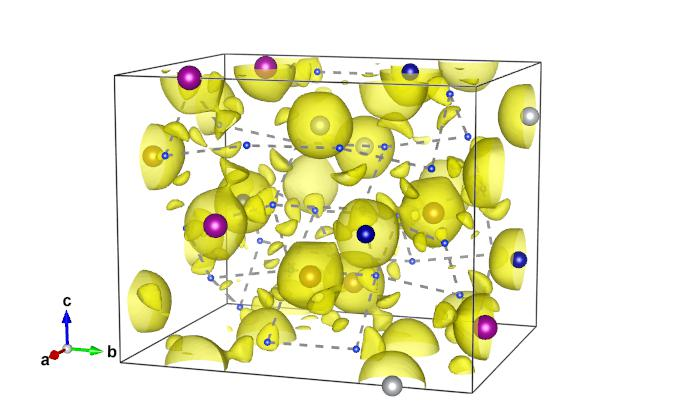
\includegraphics[width=\textwidth]{results/fesi2/B_CHGCAR.jpg}
		\caption{Structure B}
	\end{subfigure}
	\begin{subfigure}{0.5\textwidth}
		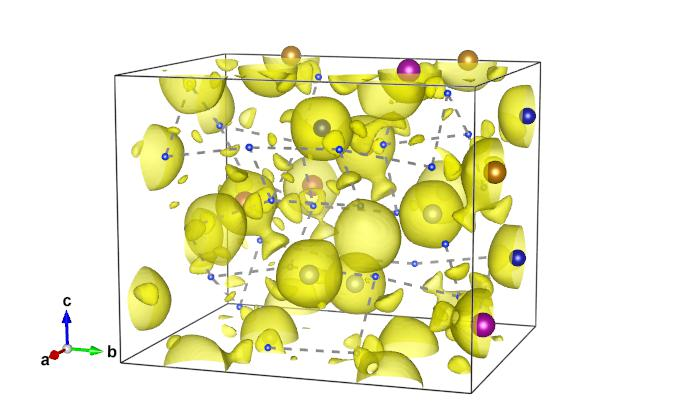
\includegraphics[width=\textwidth]{results/fesi2/C_CHGCAR.jpg}
		\caption{Structure C}
	\end{subfigure}
	\hfill
	\begin{subfigure}{0.5\textwidth}
		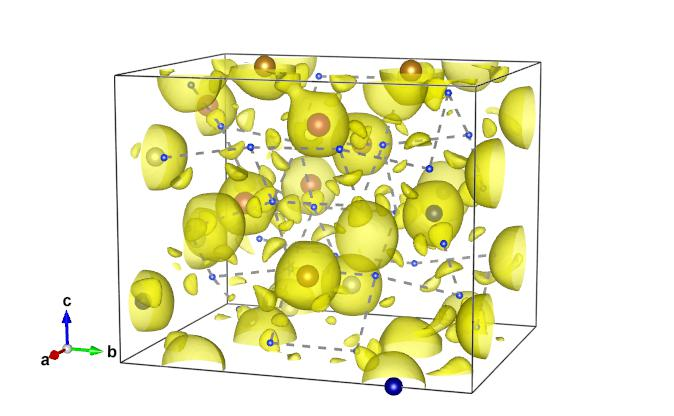
\includegraphics[width=\textwidth]{results/fesi2/D_CHGCAR.jpg}
		\caption{Structure D}
	\end{subfigure}
	\begin{subfigure}{0.5\textwidth}
		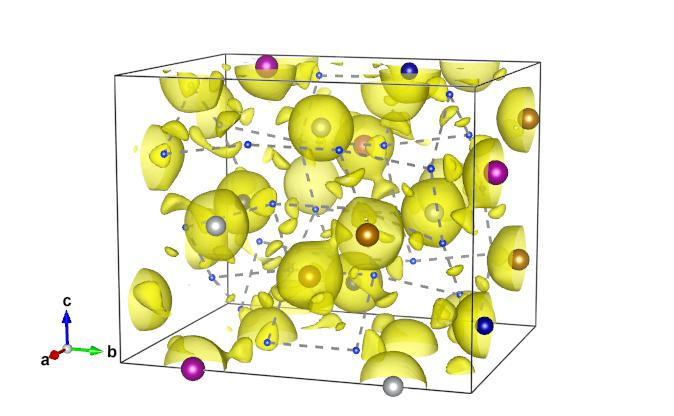
\includegraphics[width=\textwidth]{results/fesi2/E_CHGCAR.jpg}
		\caption{Structure E}
	\end{subfigure}
		\caption{Charge density}
		\label{chgcar}
\end{figure}



\textbf{Discuss CHGCAR and summarize/conclude this section. Include aspects such as stability and magnetic configuration, important here to draw parallels and discuss the results in light of high-entropy alloys, SQS, DFT and thermoelectricity. }

\textbf{Transistion into other methods and structures, present first results from SCAN and HSE06 for these 5 structures, discuss these results, but to lesser detail than PBE section. Then when finished with that, present, briefly discuss and summarize the results from all remaining structures, only include figures with good results, maybe others as well for the sake of comparison. The remaining data can be easily included in either the appendix or in a tabular format. }

\begin{figure}[H]
\centering
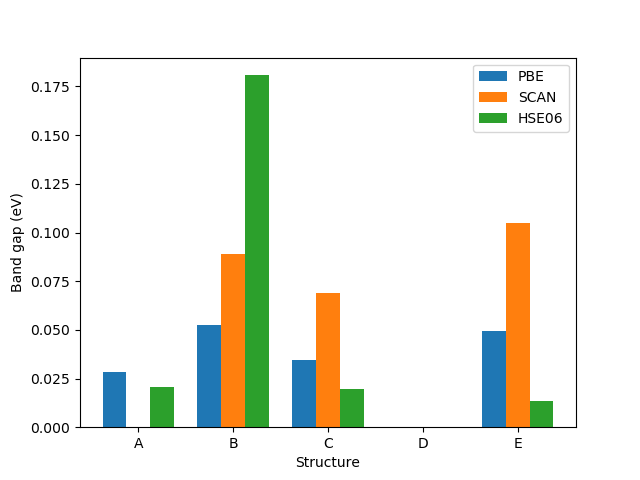
\includegraphics[scale=.7]{results/fesi2/xc_gap.png}
\caption{Band gap of CFMN (fesi2) all 5 SQSs with PBE, SCAN and HSE06}
\label{Xc_fig}
\end{figure}


Looking at the results from different functionals, we observe that the hybrid functional HSE06 more or less agree with results of the PBE functional in terms of the actual presence of the band gap, while the size of the gap is up for debate. Especially in B, where we observe a band gap greater than 0.18 eV in comparison to 0.05 eV with PBE and 0.08 with SCAN. Bellow we show the total density of states around the fermi energi $E_f$ for this structure with the HSE06 functional. 

\begin{figure}[H]
\centering
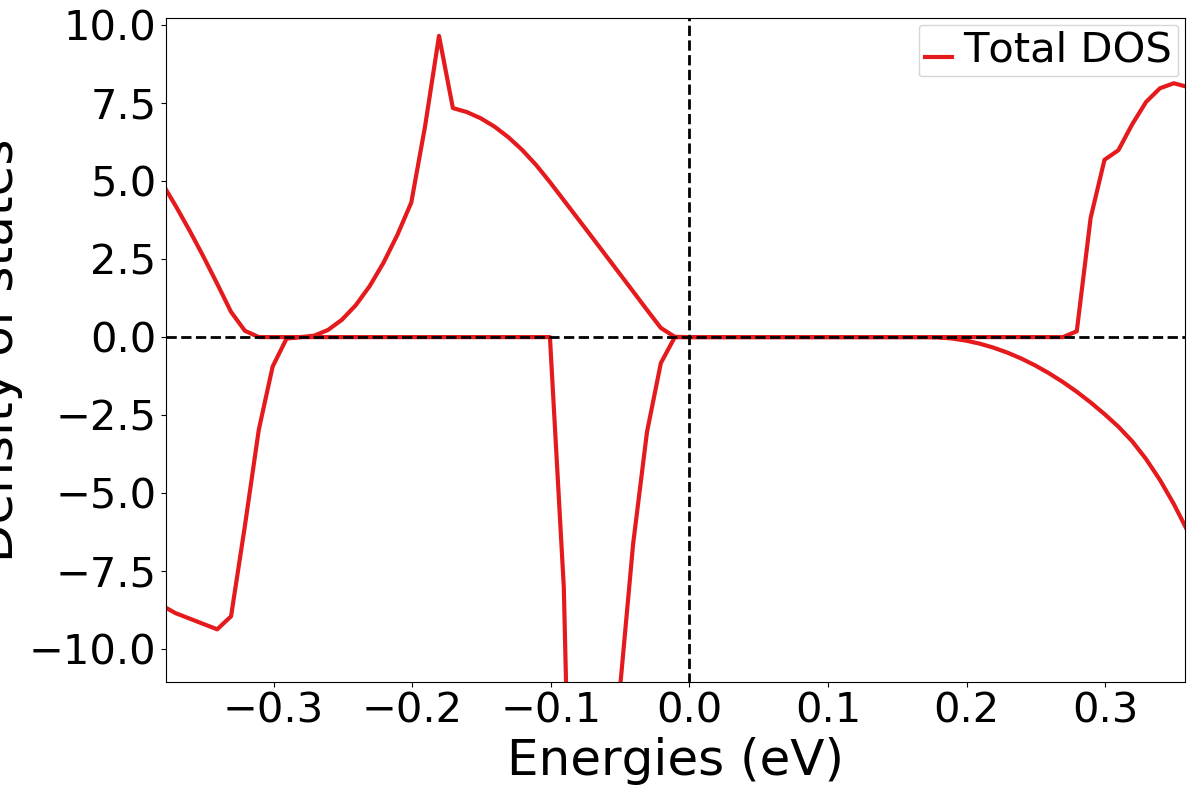
\includegraphics[scale=.3]{results/fesi2/hse06/B_DOS_zoom.png}
\caption{Density of states from HSE06 of $FeSi_2$ CFMN structure B}
\label{DOS_hse06_B}
\end{figure}

If we now compare this to the density of states of structure E,

\begin{figure}[H]
%\centering
\begin{subfigure}{0.5\textwidth}
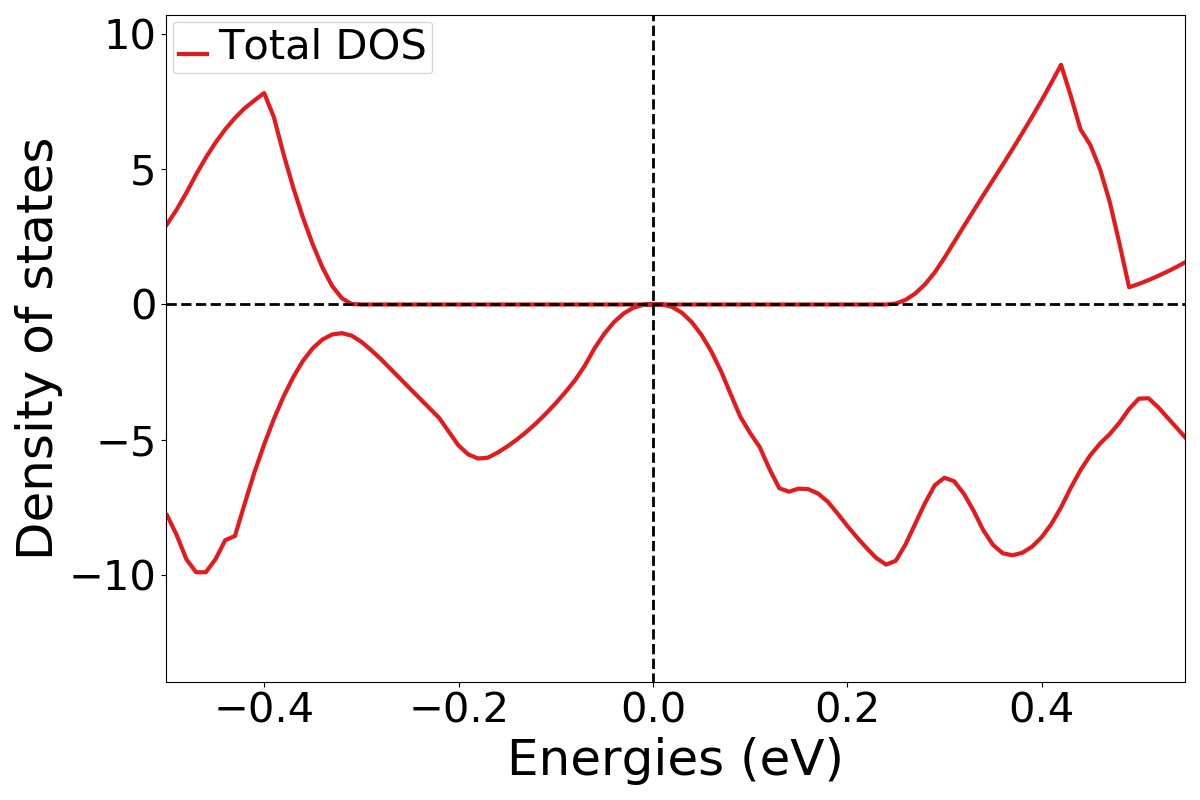
\includegraphics[width=\textwidth]{results/fesi2/hse06/E_DOS_zoom.png}
\caption{DOS $\uparrow, \downarrow$}
\end{subfigure}
\hfill
\begin{subfigure}{0.5\textwidth}
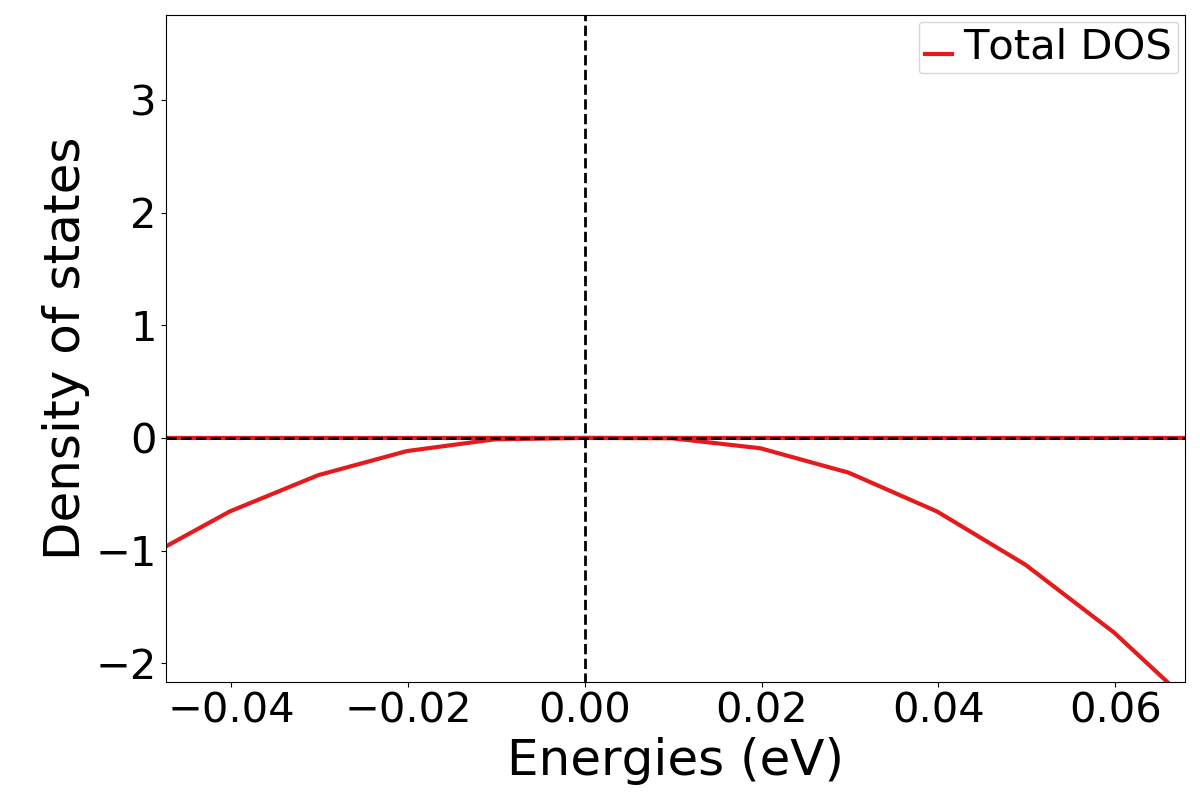
\includegraphics[width=\textwidth]{results/fesi2/hse06/E_DOS_down.png}
\caption{DOS $\downarrow$}
\end{subfigure}
\caption{The density of states of CFMN ($FeSi_2$) structure E for a) spin up and down, and b) focused on spin down}
\end{figure}


\textbf{I think its relevant and interesting to in-depth analyze structure B, D, and E. B because of large band gap. D because no band gap, and E because this well represents the other structures A and C. }
One difference is the KS eigenvalues. Str D have both partial occupancy and nonphysical occupancy, ie above 1 and bellow zero both in PBE and HSE06. This is not the case for structures that exhibited band gaps. Here we have clear transition from 1 to 0. Without having done a broad investigation of all material. This seems to be the case in other compositions and cells and permutations as well. Where both partial occupants and nonphysical occupations result in metallic structures. Calculating the band gap with strict 1 and 0 conditions, lead to small band gaps in most structures. Furthermore, in structures of Fe2Si, the difference in band where occupation transition from 1 to 0 between up and down, increases hugely compared to FeSi2 structures, talking close to 20 bands, opposed to maybe 2-5. 
